\chapter{Tools}
\section{Advanced Persistent Threat}

APT stands for Advanced Persistent Threat, a kind of sophisticated attack which requires an advanced level of expertise and aims to remain persistent on the attacked infrastructure.

The term APT can refer to a persistent attack with a specific target, or it can refer to the group that organized the attack, sometimes the group is affiliated with some sovereign state.
\\

To understand better what is an APT, we need to decompose the word: 

\textbf{Advanced:} the people behind the attack have an advanced level of expertise, resources, and money. They usually do not use known malware, but they write their malware specific to the target they want. Moreover, they can gather information on the target from the intelligence of their country of origin.

\textbf{Persistent:}  The adversary does not aim to gain access in the most number of system, but rather to have persistent access to the infrastructure. The more time they remain undiscovered in the organization's network infrastructure, the higher are the chances of lateral movement, the greater are the information they can gather. Persistent access is the key to every APT.

\textbf{Threat:} As said before, this is an organized threat, with a strategical vision of what to achieve. It is not an automatic tool that attacks everything trying to gather something. It is a meticulously planned attack that aims to obtain certain information from a given organization. \cite{apt_def}
\\

In general, APTs aim to higher-value targets like other nations or some big corporations. However, any individual can be a target. FireEye publish a report each year about the new APT campaign, the diagram below states which industry is the most attacked in the last year.\\

\begin{figure}[!h]
	\centering
	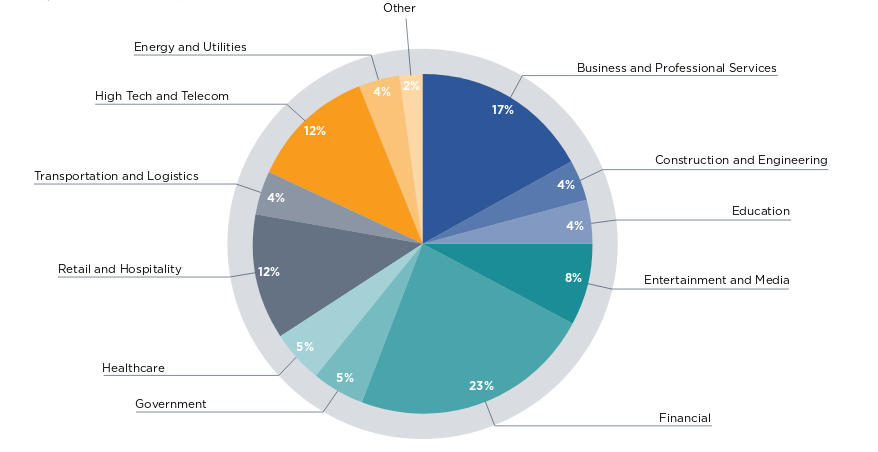
\includegraphics[width=1.0\columnwidth]{graph}
	\caption{Diagram of industry target}
\end{figure}

A point of particular concern is the retargeting, in the Americas, 63\% of the companies attacked by an APT, are attacked again last year by the same or similar group. In the Asian and Pacific areas, this is even worse, 78\% of the industries are hacked again. \cite{fireeye_mtrends} \\


\begin{figure}[ht!]
	\centering
	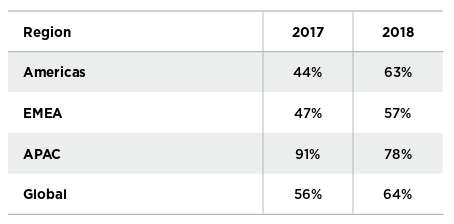
\includegraphics[width=0.5\columnwidth]{retarget}
	\caption{Retargeting divided by regions}
\end{figure}

Advanced persistent threats, contrary to regular malware, are composed of different phases, each of which has an important role. 

The attack is decomposed into smaller steps, for example, if a group of hackers wants to attack a CEO of a given company, they will not send directly to the CEO a phishing email, because it's likely that he has a complex system of security and they would be detected instantly. 

Instead, the first step would hack a person in the same company with lower permissions that can have minor defense mechanisms. Once they got the first computer, they can explore the network infrastructure of the organization, and then decide which action is the best.
They could cover their track from the log system, or locate the data they need or send a phishing email to the CEO from the owned user.\\

So how does an APT work? Fireeye described their behavior in six steps. \cite{fireeye_anatomy}


\begin{enumerate}
	\item The adversary gains access into the network infrastructure, installing a malware sent through a phishing email or by exploiting some vulnerability.
	\item Once they comprised the network, the malware scans all the infrastructure looking for other entry points or weaknesses. It can communicate with a Command \& Control server (C\&C) to receive new instructions or to send information.
	\item The malware typically establishes additional points of compromise to ensure that the attack can continue even if a position is closed.
	\item Once the attackers have a reliable connection to the network, they start dumping data such as usernames and passwords, to gain credentials.
	
	\item The malware sends the data to a server where the attackers can receive the information. Now the network is breached.
	
	\item The malware tries to cover its tracks cleaning the log system, but the network is still compromised so the adversary can enter again if they are not detected.
	
\end{enumerate}


\section{Ghidra}
Ghidra is an open-source tool for Reverse Engineering developed and by the National Security Agency (NSA). It helps analyze malicious code and malware like viruses, and can give cybersecurity professionals a better understanding of potential vulnerabilities in their networks and systems \cite{ghidra}
\begin{wrapfigure}{L}{0.35\textwidth}
	\centering
	
\includegraphics[width=0.35\textwidth]{ghidra}
	
\end{wrapfigure}


Usually, reverse engineering is the process of analyzing something to understand how it works. In the case of a program written in Java or C or C++, the code will be readable by a human but not bt a computer. It needs to be compiled in a language understandable by the network, but once it is compiled, we can no more read it. \\

To understand how the program works, we need a toolkit to take it apart, and this is what Ghidra does. There are a lot of tools in the market that can do the same thing, in different ways, some of them are open-source and free, other you need to pay a license. 

We choose to use Ghidra because it is free, and it offers the possibility of writing scripts to run against the binaries analyzed. In this way, we extracted all the necessary information automatically from the APT binaries.
\section{Scikit-learn}

Scikit-learn is a Python module integrating a wide range of state-of-the-art machine learning algorithms for medium-scale supervised and unsupervised problems. 

It is open-source, commercially usable, and contains many modern machine learning algorithms for classification, regression, clustering, feature extraction, and optimization.
For this reason, Scikit-Learn is often the first tool in a Data Scientists toolkit for machine learning of incoming data sets. \cite{scikit-learn}
